% !TeX spellcheck = it_IT
\section{WPAN}

Lo standard 802.15 comprende un insieme di tecnologie per la comunicazione a corto raggio.

\subsection{Bluetooth}

Standard 802.15.1. Si compone di reti chiamate \textbf{piconet}, all'interno della rete si ha un \textbf{master} che controlla la piconet e uno o più \textbf{slave} controllati.

Si tratta di comunicazione short range (10-50m), usa la banda ISM $2.4GHz$, data rate $2.1Mbps$-$24Mbps$.

\subsubsection{Piconet \& Scatternet}

Una piconet è composta da \textbf{master} e 
\begin{itemize}
    \item \textbf{Active Slave AS:} membro attivo della piconet, con un Active Member Address AMA di 3 bit assegnato dal master
    
    \item \textbf{Parked Slave PS:} membro della piconet temporaneamente disattivato, con un Parked Member Address PMA di 8 bit
    
    \item \textbf{Standby Slave SS:} membro non sconosciuto ma scollegato, senza indirizzo
\end{itemize}

\paragraph{Scatternet:} Un dispositivo può appartenere a più piconet differenti, portando a una scatternet. Le due piconet rimangono completamente autonome. Nel caso le due piconet usino la stessa frequenza per comunicare, si ha CDMA per evitare interferenze.

\subsubsection{Architettura dei protocolli}

Ci sono dei protocolli definiti \textit{core}, ovvero necessariamente implementati all'interno di tutti i dispositivi Bluetooth.

\paragraph{Bluetooth radio:} Livello fisico, specifica l'interfaccia radio: quali frequenze usare, gestisce il frequency hopping, schema di modulazione e potenza di trasmissione.

Per gestire le scatternet si usa FH-CDMA, anche in caso usino la stessa frequenza si ha il CDMA.

Per comunicare all'interno di una piconet vengono usate: 
\begin{itemize}
    \item Frequency Hopping FH: frequenza decisa dal master, determinata in base al numero di slot passati
    
    \item Time Division Duplex TDD: la comunicazione è a slot alternati master-slave, ogni $625\mu s$; la dimensione dei messaggi è di 1, 3 o 5 slot, per mantenere l'alternanza
    
    \item Time Division Multiple Access TDMA: per gestire più dispositivi nello stesso momento; il master decide chi può comunicare in quale slot di tempo
\end{itemize}

\paragraph{Baseband:} Si occupa di stabilire la connessione con la piconet, gestire l'indirizzamento, formattazione dei pacchetti, gestire le tempistiche di comunicazione e potenza di trasmissione.

Offre due tipologie di servizio (canali logici): 
\begin{itemize}
    \item \textbf{Synchronous Connection-Oriented Link (SCO)} point-to-point: canale bidirezionale $64kbps$, tipicamente audio/voce; il master riserva una coppia di slot adiacenti a intervalli regolari; fino a 3 canali SCO attivi contemporaneamente; traffico real time. Garantiscono un bit rate fisso, per casi delay-sensitive.
    
    \item \textbf{Asynchronous Connectionless Link (ACL)} point-to-multipoint: occupano tutti gli slot rimanenti, traffico best effort; qualità maggiore senza nessuna garanzia
\end{itemize}

Alcuni dei campi all'interno dei pacchetti:
\begin{itemize}
    \item Accesso code 72 bit: utilizzato per sincronizzazione e identificazione. Può essere di 3 tipi: Channel Access Code (CAC, identifica la piconet), Device Address Code (DAC, indirizzo dello slave), Inquiry Address Code (IAC, usato per trovare l'indirizzo di un dispositivo vicino)
    
    \item AMA: indirizzo del membro attivo 
    
    \item Type: tipo del pacchetto
    
    \item ARQN: 1 ack, 0 nack
    
    \item SEQN: 1 bit di sequence number
\end{itemize}

ARQN e SEQN sono 2 bit e sufficienti per il controllo degli errori. La sequenza di invio tipica è: 
\begin{itemize}
    \item master invia un pacchetto con SEQN $s$
    
    \item lo slave risponde con ACK e SEQN $s$
\end{itemize}

Per la trasmissione successiva si inverte il SEQN. Problemi possibili: 
\begin{itemize}
    \item slave non riceve il pacchetto: risponde con SEQN corretto e NACK; il master re invia il pacchetto
    
    \item master non riceve ack: ritrasmette con lo stesso SEQN, lo slave capisce che deve ritrasmettere l'ack dato che il SEQN è uguale al precedente
\end{itemize}

\paragraph{Link Manager Protocol:} "Manager" del collegamento, si occupa di configurare i collegamenti tra dispositivi, gestire i collegamenti attivi e funzionalità di sicurezza e cifratura. Protocollo solamente di controllo, niente dati.

Transizioni di stato:
\begin{center}
    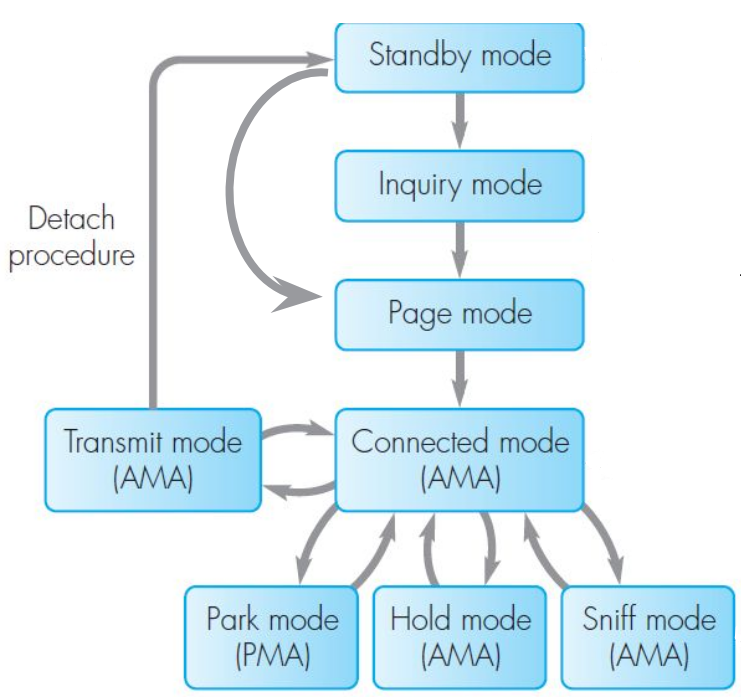
\includegraphics[width=0.45\linewidth]{../img/wpan/lmpst}
\end{center}

Appena acceso il dispositivo entra in \textbf{standby mode}, nessuna piconet, minimo consumo.

Il master invia periodicamente 32 messaggi consecutivi su canali standard, i quali contengono un IAC packet. Gli slave in \textbf{inquiry mode} ascoltano periodicamente i canali aspettando un IAC packet.

Ogni slave ascolta sulle frequenze di wake-up, una volta trovata una trasmissione si può sincronizzare al clock del master, fare random backoff di qualche slot, per poi rispondere. Il master risponde con DAC, AMA e sequenza per il FH, su 16 dei 32 canali. Lo slave risponde con DAC e ACK. 

In fase di \textbf{paging}, il master invia messaggi di paging per richiamare il dispositivo target, fornire tutti i dati di sincronizzazione necessari e stabilire definitivamente la connessione.

Altri stati: un dispositivo può essere: 
\begin{itemize}
    \item Connected mode: connesso senza trasmettere
    
    \item Transmit mode: quando deve trasmettere
    
    \item Sniff mode: non ascolta tutti gli slot, mantiene AMA
    
    \item Hold mode: ascolta solo canali SCO, mantiene AMA
    
    \item Park mode: rilascia l'AMA, rimane membro della piconet, riceve un PMA. Ascolta periodicamente messaggi in broadcast, rimane sincronizzato
\end{itemize}
Le ultime 3 sono modalità di power saving. 

\paragraph{Logical Link Control and Adaptation Protocol L2CAP:} Primo livello implementato a livello software. Si occupa di adattare i protocolli di livello superiore al livello baseband e astrarre le feature esposte dai livelli inferiori.

Supporta solo canali ACL e offre 3 tipi di canali logici: 
\begin{itemize}
    \item \textbf{Connectionless:} unidirezionale, senza connessione
    
    \item \textbf{Connection-oriented:} bidirezionale, orientato alla connessione, supporta QoS
    
    \item \textbf{Signaling:} bidirezionale, usato per messaggi di controllo
\end{itemize}

Gestisce anche segmentazione e ricostruzione dei frame inviati a livello baseband.

Il tipo di pacchetto viene identificato dal campo Channel Identifie CID: $=1$ signaling, $=2$ connectionless, $\geq 64$ connection-oriented.

\paragraph{Service Discovery Protocol SDP:} Protocollo client-server, il client può richiedere al server: 
\begin{itemize}
    \item ricerca di un servizio
    
    \item browse dei servizi disponibili sul dispositivo
\end{itemize}
Generalmente master chiede, slave risponde.

\subsection{BLE}

Vuole ridurre i consumi, semplificare il sistema di comunicazione.

Introduce nuove strutture di comunicazione: 
\begin{itemize}
    \item \textbf{Broadcast}: chi è in range ascolta un broadcaster
    
    \item \textbf{Mesh:} ogni dispositivo può essere connesso a molteplici altri
\end{itemize}

Aggiunge servizi di positioning, permette di rilevare presenza, distanza e direzione di un dispositivo.

Stessa banda ISM $2.4GHz$, ma 40 canali al posto che 79.

\subsubsection{Architettura}

Il fisico cambia, il resto è equivalente a BT 2.1.
\begin{center}
    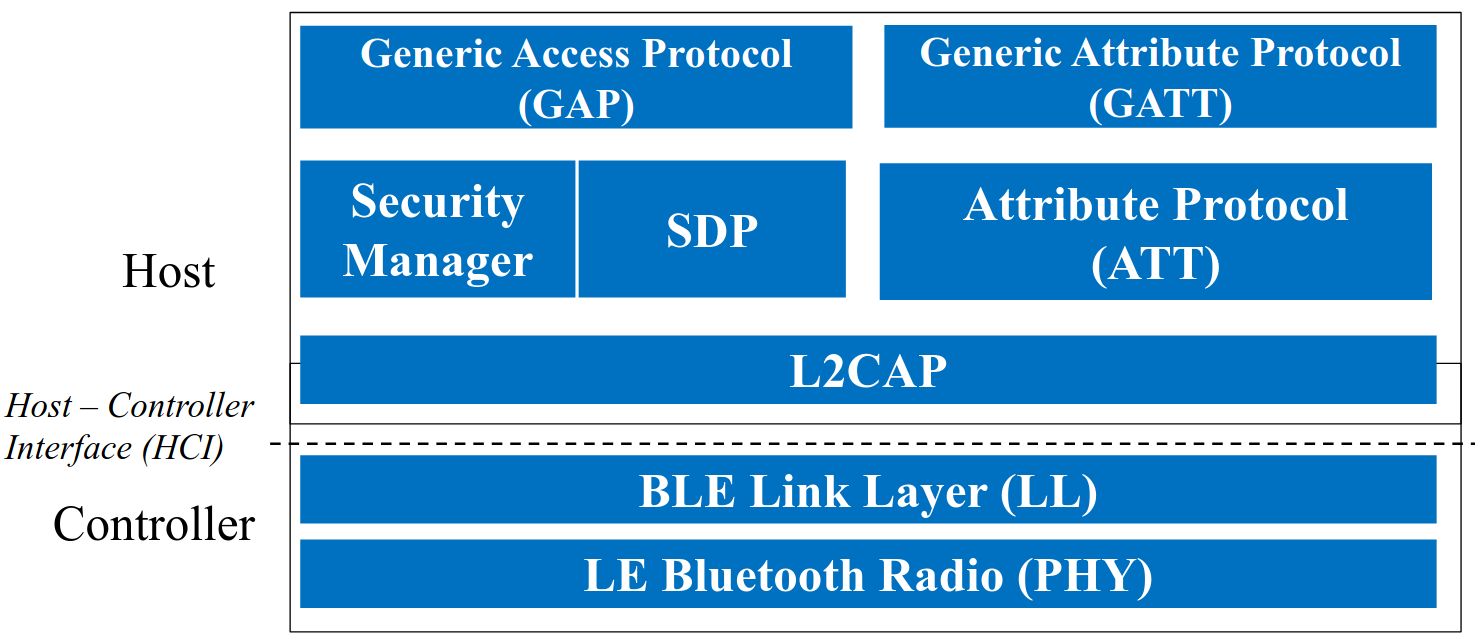
\includegraphics[width=0.7\linewidth]{../img/wpan/blearch}
\end{center}

\paragraph{BLE Radio (PHY):} 37 canali usati per data, ultimi 3 per advertising.

\paragraph{Generic Attribute Profile GATT:} Permette scambio di dati strutturati tra client che richiedono e server che offrono servizi tramite profili. I ruoli non sono fissi, ogni profilo ha dati e caratteristiche associate.

\paragraph{General Access Protocol GAP:} Un'applicazione può decidere uno dei ruoli fondamentali definiti da GAP: 
\begin{itemize}
    \item \textbf{Broadcaster:} spedisce dati in modo connectionless come pacchetti di advertising
    
    \item \textbf{Observer:} riceve pacchetti di advertising connectionless
    
    \item \textbf{Peripheral:} opera in slave (advertiser) mode a livello di link layer 
    
    \item \textbf{Central:} opera in master (initiator) mode a livello di link layer
\end{itemize}

\paragraph{Creazione connessione unicast:} Il master ascolta, lo slave è l'advertiser, vuole essere trovato mandando advertising packets. Una volta che il master (initiator) ascolta un messaggio, invia una connection request nello slot di tempo successivo, contenente anche le informazioni per il FH. 

\paragraph{Connessione broadcast:} Per quando un broadcaster ha solo interessa a inviare dati. Gli observer ascoltano i canali di advertising per i messaggi del broadcaster.

Lo scanning può essere passivo oppure attivo, in cui vengono richiesti dati in unicast al dispositivo di broadcast tramite i canali di advertising.

\subsubsection{BLE State Machine}

Tutti partono dallo \textbf{standby}, possono andare a:
\begin{itemize}
    \item \textbf{Advertising:} lo slave si annuncia per cercare la piconet, non è più il master che cerca
    
    \item \textbf{Initiating:} vengono ascoltati i messaggi di advertising
    
    \item \textbf{Isochronous broadcasting:} periodico broadcasting di informazioni 
    
    \item \textbf{Scanning:} il dispositivo si mette in ascolto
\end{itemize}

\paragraph{Advertising:} Ogni certa quantità di tempo, viene inviato un advertising event su uno o più dei canali di advertising. Il tempo è determinato da due parametri: \texttt{advInterval} stabilito e \texttt{advDelay} più breve e casuale.

\subsection{ZigBee}

Standard 802.15.4, cerca principalmente affidabilità, basso costo e complessità, bassissimo consumo, scalabilità. Usa le bande $2.4GHz$ e $915$/$868MHz$.

\paragraph{Topologia di rete:} Si possono avere topologie a stella, albero o mesh, quindi anche multi-hop (serve routing).

\paragraph{Classi di nodi:} Ci sono due macro classi di nodi:
\begin{itemize}
    \item \textbf{Full Function Device FFD:} Un coordinatore e uno o più router, possono fare instradamanto
    
    \item \textbf{Reduced Function Device RFD:} end device, possono solo comunicare e ricevere dati; ridotta complessità e consumo
\end{itemize}

\paragraph{Tipologie di dati:} In base al caso d'uso: 
\begin{itemize}
    \item \textbf{periodici:} inviati dopo un intervallo di trasmissione fissato
    
    \item \textbf{intermittenti:} comunicati in base a un evento; asincroni
    
    \item \textbf{ripetitivi e a bassa latenza:} allocazione di time slot
\end{itemize}

\subsubsection{Architettura}

\paragraph{Livello PHY:} Vengono specificati tipo di modulazione e spread spectrum per ognuna delle 3 bande possibili.

Multiplexing sui canali all'interno della banda, spread spectrum DSSS per la comunicazione. I data rate sono sempre molto limitati.

\paragraph{Livello MAC:} Si occupa di
\begin{itemize}
    \item gestire l'invio dei beacon per il coordinatore, sincronizzazione con i beacon del coordinatore per gli altri 
    
    \item (dis)associazione alla PAN ascoltando i beacon
    
    \item accesso al canale tramite CSMA/CA
    
    \item MAC Address 
    
    \item gestione del duty cycle
\end{itemize}

Si possono avere due tipi di trasmissioni: 
\begin{itemize}
    \item diretta: bidirezionale dispositivo e coordinatore
    
    \item indiretta: solo da coordinatore verso il dispositivo
\end{itemize}

\paragraph{Modalità di trasferimento:} Sono due possibili: 
\begin{itemize}
    \item \textbf{Unslotted CSMA/CA}, senza l'ausilio di beacon; i dispositivi accedono usando CSMA/CA, senza vincoli di slot; si ripete la fase di backoff finché non riesce a trasmettere
    
    \item \textbf{Slotted CSMA/CA}, con beacon
\end{itemize}

\paragraph{Slotted CSMA/CA:} Si fonda sull'invio di beacon da parte del coordinatore; vengono usati per
\begin{itemize}
    \item sincronizzare i dispositivi
    
    \item organizzare i periodi di trasmissione
    
    \item gestire la trasmissione indiretta, nei beacon viene trasmessa la lista di dispositivi che hanno frame pendenti
\end{itemize}

Il tempo totale tra un beacon e l'altro è detto \textbf{superframe}, rappresenta l'organizzazione logica della comunicazione. Si ha un duty cycle, si alternano periodi di attività e inattività, in cui viene spenta la radio.

L'\textbf{intervallo tra beacon} è
$$ aBaseSuperframeDuration \cdot 2^{BO}$$
simboli, dove $aBaseSuperframeDuration = 960$ simboli e il Beacon Order $BO$ va da 0 a 14.

La \textbf{durata del superframe} invece è
$$ aBaseSuperframeDuration \cdot 2^{SO} $$
dove il Superframe Order $SO$ è sempre un valore 0-14.

Il rapporto tra i due fornisce il duty cycle.

Il superframe viene di viso in slot con diversi tipi di accesso: 
\begin{itemize}
    \item \textbf{Contention Access Period CAP:} accesso al canale usando CSMA/CA. Canale a contesa, per capire lo stato del canale: 
    \begin{itemize}
        \item viene scelto un intero casuale nell'intervallo $[0, 2^{BE} - 1]$, dove il Backoff Exponent $BE$ è un parametro, e viene atteso quel numero di slot (20 simboli); se il conteggio viene interrotto, riprende al superframe successivo
        
        \item Dopo l'attesa, vengono fatti $CW$ Clear Channel Assessment, dove Contention Window $CW$ è un parametro
        
        \item Se dopo i CCA il canale è libero comincia a trasmettere
        
        \item Se il canale risulta occupato, si allarga la finestra del random backoff incrementando di 1 $BE$ e il numero di backoff $NB$
        
        \item Se $NB = 4$: transmission failure
    \end{itemize}
    
    \item \textbf{Contention Free Periodo CFP:} intervallo per le comunicazioni con banda riservata tramite Guaranteed Time Slot (campo del beacon)
\end{itemize}